\documentclass[11pt]{report}
\usepackage[a4paper, width=6in, height=9.2in]{geometry}
\usepackage[portuguese]{babel}
\usepackage[utf8]{inputenc}
\usepackage{listings}
\usepackage{color}
\usepackage{setspace}
\usepackage{hyperref}
\usepackage{acro}
\usepackage{amsmath}
\usepackage{amsthm}
\usepackage{graphicx}
\usepackage{subcaption}
\usepackage{cancel}
\usepackage{tikz}
\usepackage{color}
\usepackage{float}
\usepackage{titlesec}
\usepackage{todonotes}
\usepackage{minted}

\usemintedstyle{autumn}

\setstretch{1.3}
\renewcommand{\arraystretch}{1.3}

% Ajustar o espaçamento antes de capítulos, indíce, etc.
\titleformat{\chapter}[display]{\normalfont\huge\bfseries}{\chaptertitlename\ \thechapter}{20pt}{\Huge}
\titlespacing*{\chapter}{0pt}{-16pt}{30pt}


\begin{document}

% Capa
\title{Conceção e otimização de modelos de \textit{Machine Learning}\\
       \textbf{Trabalho Prático}\\
       Dados e Aprendizagem Automática}

\author{João Paulo Machado Abreu \\ pg53928
        \and João Pedro Dias Faria \\ pg53939
        \and Ricardo Cardoso Sousa \\ pg54179
        \and Rui Pedro Guise da Silva \\ pg54213}

\date{10 de janeiro de 2024}

% Exibir título, autor e data especificados
\maketitle


% Índice
\pagenumbering{roman}
\tableofcontents

% Capítulos e subcapítulos
\newpage
\pagenumbering{arabic}
\chapter{Introdução}
\paragraph{}
Este relatório inclui os resultados do trabalho prático realizado no âmbito da unidade curricular de Dados e Aprendizagem Inteligente como forma de aprofundar o conhecimento sobre a matéria lecionada ao longo do semestre. O objetivo deste trabalho foi desenvolver modelos de aprendizagem automática para a resolução de problemas reais.

Os primeiros modelos criados foram desenvolvidos para prever a produção de energia solar. Para isso, foi utilizado um conjunto de \textit{dataset} fornecidos pela equipa docente que contêm informações sobre as condições meteorológicas, a temperatura e a radiação solar dos últimos três anos. Os modelos foram desenvolvidos utilizando técnicas de classificação, tendo como resultado final a previsão da quantidade de energia solar produzida em cada dia.

Os restantes modelos foram desenvolvido para prever o nível de \textit{burnout} em trabalhadores. Para isso, foi utilizado um \textit{dataset} escolhido pelo grupo que contém informações sobre as cargas de trabalho, os escalões e o nível de fadiga mental dos trabalhadores. Os modelos foram desenvolvidos utilizando técnicas de regressão, tendo como resultado final uma pontuação que indica o nível de \textit{burnout} de cada trabalhador.

\section{Metodologia Utilizada}
\paragraph{}
Para a realização do trabalho prático, o nosso grupo optou por seguir uma metodologia SEMMA (Sample, Explore, Modify, Model, Assess) em ambos os \textit{datasets} apresentados. A utilização desta metodologia é importante para o desenvolvimento de modelos por diversas razões. Esta metodologia fornece uma estrutura para o processo de desenvolvimento, o que ajuda a organizar o trabalho e a evitar erros. A metodologia garante, ainda, que o modelo seja desenvolvido de forma consistente, o que facilita a replicação do modelo em outros contextos. E por fim, a metodologia ajuda a identificar problemas nos dados ou no modelo, o que pode levar a melhorias no desempenho do modelo. Ao longo deste relatório será possível verificar o trabalho desenvolvido em cada uma das fases de desenvolvimento, desde a análise e compreensão dos dados até à avaliação dos modelos.

\chapter{\textit{Dataset} da Competição: Produção Energética e Sustentabilidade}

\section{Descrição}
\paragraph{}
O \textit{dataset} de competição, é um cojunto de \textit{datasets} disponibilizados pela equipa docente, apresentando diversos dados referentes à produção energética de determinados painéis solares e à situação meteorológica na cidade de Braga, para cada hora e dia do ano de 20021 até ao ano de 2023.
Os \textit{datasets} utilizados nesta competição contêm um elevado conjunto de \textit{features} sendo de destacar a \textit{feature} Injeção na rede (kWh). Esta \textit{feature} é considerada o nosso target, uma vez que, o problema que se impõe, com estes \textit{datasets}, é prever a quantidade de energia, em kWh, produzida por painéis e injetada, em redes elétricas, a cada hora do dia. 

\section{Exploração de dados}

\subsection{Tipos de dados}
\paragraph{}
Através da método \textit{info()}, conseguimos verificar o tipo de cada coluna, sendo possível identificar 5 colunas do tipo \textit{object} (Data, Injeção na rede (kWh), dt\_iso, city\_name e weather\_description), que serão tido em conta na preparação de dados para poderem ser utilizados nos modelos criados.

\begin{figure}[H]
    \centering
    \centerline{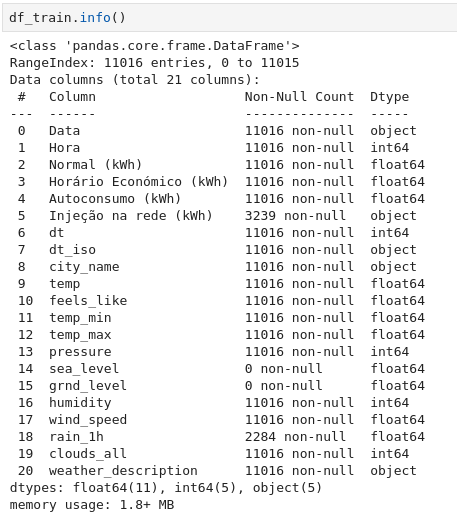
\includegraphics[width=0.5\textwidth]{Imagens/Competição/info_competicao.png}}
    \caption{Método \textit{info()}}
    \label{fig: info_competicao}
\end{figure}

\subsection{\textit{Missing values}}
\paragraph{}
Na análise dos dados foi verificada a existência de \textit{missing values} nos dados de treino nas colunas Injeção na rede (kWh), sea\_level, grnd\_level e rain\_1h. Já nos dados de teste para além destas últimas 3 colunas, os dados que acrescentamos apresentavam \textit{missing values} nas colunas temp\_min e temp\_max.

\begin{figure}[H]
    \centering
    \centerline{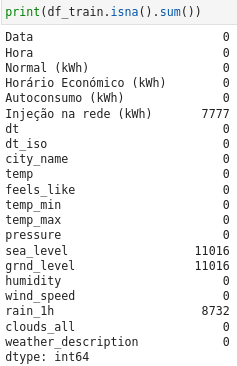
\includegraphics[width=0.3\textwidth]{Imagens/Competição/missing_values.png}}
    \caption{\textit{Missing values}}
    \label{fig: missing_values}
\end{figure}


\section{Preparação de dados}

\subsection{\textit{Feature} engeneering sobre as datas}
\paragraph{}
Através da coluna 'Data' o grupo aplicou técnicas de \textit{feature} engineering para extrair novas \textit{features} a partir desta. A partir desta retiramos então o ano, mês e dia com o objetivo de verificar se algum destes atributos tinha influência na nossa \textit{label}.

\subsection{Tratamento de \textit{missing values}}
\paragraph{}
Para os \textit{missing values} de Injeção na rede (kWh) e rain\_1h o grupo considerou que a falta de valores nas colunas deve-se ao facto de não ter havido injeção na rede ou chuva, deste modo todos os valores em falta foram preenchidos com valor 0 para representar a inexistência de injeção ou chuva.
Já para as \textit{features} sea\_level, grnd\_level, uma vez que toda a coluna apresentava \textit{missing values} decidimos remover ambas as colunas uma vez que, as mesmas, não acrescentam informação importante para treinar os nossos modelos.

Removemos ainda as colunas 'dt' e 'dt\_iso', uma vez que sendo um valor distinto para cada linha, não representa nenhuma informação relevante para o treino dos nossos modelos. Pela razão oposta foi também retirada a \textit{feature} city\_name por ser um valor único para todas as linhas e, por essa razão, não representar informação relevante para o treino dos nossos modelos.

\subsection{Tratamento de dados categóricos}
\paragraph{}
Para tratamento do dados categóricos restantes, weather\_description e Injeção na rede (kWh), visto que ambas as colunas têm uma certa ordem (categóricos ordinais), os valores de ambas as colunas foram substituídos por números inteiros relacionados com a sua ordem prévia.
As associações utilizadas podem ser observadas na seguinte imagem:

\begin{figure}[H]
    \centering
    \begin{minted}[fontsize=\footnotesize, xleftmargin=16pt, breaklines=true, breakanywhere=true]{python}
replace_map = {'Injeção na rede (kWh)': {'None': 0, 'Low': 1, 'Medium': 2, 'High': 3, 'Very High': 4}}
    \end{minted}
    \caption{\textit{Label 'Injeção na rede'}}
    \label{fig1}
\end{figure}

\begin{figure}[H]
    \centering
    \begin{minted}[fontsize=\footnotesize, xleftmargin=16pt, breaklines=true, breakanywhere=true]{python}
replace_map = {'weather_description': {'sky is clear': 1,'few clouds': 2, 'scattered clouds': 3,'broken clouds': 4,'overcast clouds': 5, 'light rain': 6, 'moderate rain': 7, 'heavy intensity rain': 8}}
    \end{minted}
    \caption{\textit{Feature 'weather description'}}
    \label{fig2}
\end{figure}

Foram removidos os atributos 'date\_day' e 'date\_year' por não apresentarem uma correlação relevante com nenhuma das restantes \textit{features}, não acrescentando qualquer informação pertinente ao treino dos modelos.
A \textit{feature} 'weather\_description' foi removida por apresentar uma correlação forte com o atributo 'clouds\_all', decidimos manter esta última por apresentar os valores originais sem nenhum tratamento específico, sendo mantido assim a naturalidade dos dados.

Através do \textit{lineplot} que relaciona a hora com a nossa \textit{target}, o grupo decidiu criar um novo atributo que representasse a fase do dia, isto porque a injeção na rede varia consoante a hora do dia. Esta nova coluna foi criada analisando este gráfico:

\begin{figure}[H]
    \centering
    \centerline{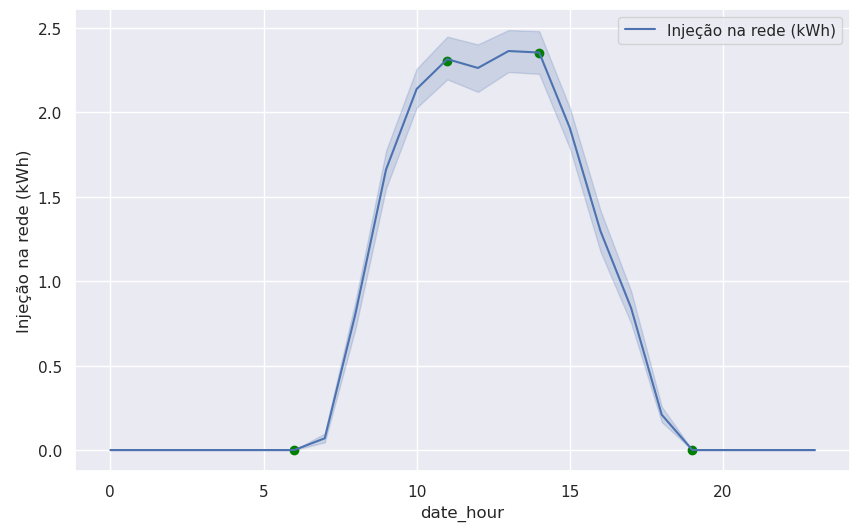
\includegraphics[width=1\textwidth]{Imagens/Competição/line_plot_competicao.png}}
    \caption{Relação da \textit{feature Injeção na Rede} com a \textit{feature date\_hour}}
    \label{fig}
\end{figure}

E com auxilio da seguinte função:
\begin{minted}[fontsize=\footnotesize, xleftmargin=16pt, breaklines=true, breakanywhere=true]{python}
def fase_do_dia(hour):
    if hour <= 6 and hour >= 19:
        return 1
    elif hour <= 11 and hour >= 6:
        return 2
    elif hour <= 14 and hour >= 11:
        return 3
    else:
        return 4
\end{minted}

\section{Modelação}
\paragraph{}
Finalmente, após uma exploração e preparação de dados cuidadosa, partimos então para a criação dos nossos modelos. Para a criação de bons modelos com o objetivo que estes realizassem boas previsões tantos para o nosso \textit{dataset} como para dados desconhecidos, o grupo tentou evitar tanto situações de underfitting como overfitting.
Com este fim o grupo decidiu dividir os dados de treino em 2 conjuntos distintos, um para treinar os modelos e outro para os testar. Foi decidido então que a percentagem de cada um seria 80\% e 20\% respetivamente.

\begin{minted}[fontsize=\footnotesize, xleftmargin=16pt, breaklines=true, breakanywhere=true]{python}
X = df_train.drop(['Injeção na rede (kWh)'], axis=1)
y = df_train['Injeção na rede (kWh)']
\end{minted}

\begin{minted}[fontsize=\footnotesize, xleftmargin=16pt, breaklines=true, breakanywhere=true]{python}
X_train_p, X_test_p, y_train_p, y_test_p = train_test_split(X, y, test_size=0.2, random_state=2023)
\end{minted}

Sabendo que o problema em mão é de classificação foram criados então os seguintes modelos:

\subsection{Árvores de Decisão}
\paragraph{}
Com o primeiro modelo criado decidimos utilizar Decision Tree, uma vez que foi um dos primeiros modelos abordados durante esta UC. Para além disso são também um dos modelos mais usados perante problemas de classificação.

Numa perspetiva mais de programação, foi utilizado DecisionTreeClassifier presente na biblioteca Sklearn e para obter os melhores hiperparâmetros, recorremos ao auxílio de GridSearchCV.

\begin{minted}[fontsize=\footnotesize, xleftmargin=16pt, breaklines=true, breakanywhere=true]{python}
param_grid_dt = { 'criterion': ['gini','entropy','log_loss'], 'max_depth': [5,6,7,8], 'min_samples_split': [2,3,4], 'min_samples_leaf': [1,2,3,4] }
estimator_dt = DecisionTreeClassifier(random_state=2021)
grid_dt = GridSearchCV(estimator_dt, param_grid_dt, refit=True, verbose=0)
\end{minted}

O melhor modelo obtido foi:
\begin{figure}[H]
    \centering
    \centerline{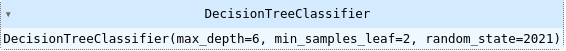
\includegraphics[width=0.7\textwidth]{Imagens/Competição/dt.png}}
    \label{fig: dt}
\end{figure}

e feita a previsão para os dados de teste criados foi obtido então uma accuracy de 86.66\%. Através do classification report analisamos ainda outras métricas como f1-score e recall.

\subsection{Random Forest}
\paragraph{}
De seguida decidimos utilizar Random Forest, algoritmo que tínhamos já utilizado durante a licenciatura e foi também abordado no final desta UC como técnica de ensemble learning.
O benefício que estas trazem relativamente às árvores de decisão, é que as random forest têm uma tendência inferior a overfitting sendo um dos aspetos que pretendemos atenuar.

Usamos então RandomForestClassifier e, mais uma vez, com o auxílio de GridSearchCV descobrimos os melhores hiperparâmetros.

\begin{minted}[fontsize=\footnotesize, xleftmargin=16pt, breaklines=true, breakanywhere=true]{python}
param_grid_dt2 = { 'n_estimators': [150,200,250], 'max_depth': [7,8,9], 'min_samples_split': [2,3,4], 'min_samples_leaf': [1,2,3] }
estimator_dt2 = RandomForestClassifier(bootstrap=False, random_state=2022)
grid_dt2 = GridSearchCV(estimator_dt2, param_grid_dt2, refit=True, verbose=0)
\end{minted}

O melhor modelo obtido apresenta os seguintes hiperparâmetros:
\begin{minted}[fontsize=\footnotesize, xleftmargin=16pt, breaklines=true, breakanywhere=true]{python}
{'max_depth': 9, 'min_samples_leaf': 1, 'min_samples_split': 3, 'n_estimators': 150}
\end{minted}

Feita a previsão para o os dados de teste criados obtemos 88.61\% accuracy, um resultado visivelmente melhor que o anteriormente obtido.
Estas melhorias são também visíveis nas métricas disponibilizadas por classification report.
Concluímos então que a random forest generaliza melhor que as decision tree, porém são modelos que requerem um custo computacional mais elevado.

\subsection{Máquinas de Vetores de Suporte (SVM)}
\paragraph{}
Decidimos ainda explorar SVM, para ver como se comportavam perante o nosso \textit{dataset}.
Como nos anteriores modelos foi utilizado GridSearchCV para descobrir os melhores hiperparâmetros do SVC.

O melhor modelo obtido apresenta então os seguintes hiperparâmetros:
\begin{minted}[fontsize=\footnotesize, xleftmargin=16pt, breaklines=true, breakanywhere=true]{python}
param_grid = {'C': [0.1,1,10,100,1000], 'gamma': [1,0.1,0.01,0.001,0.0001], 'kernel': ['rbf','linear']}
\end{minted}

E os seguintes resultados:
\begin{minted}[fontsize=\footnotesize, xleftmargin=16pt, breaklines=true, breakanywhere=true]{python}
{'C': 1000, 'gamma': 0.001, 'kernel': 'rbf'}
\end{minted}

Como já esperávamos este modelo foi o que nos trouxe uma accuracy inferior no entanto conseguiu prever 85.66\% dos valores corretos.

\subsection{XGBoost}
\paragraph{}
Uma vez lecionada, procedemos à implementação de novas técnicas de ensemble learning procedendo à implementação de XGBoost.

Mais uma vez utilizamos GridSearchCV para descobrir os melhores hiperparâmetros para XGBClassifier.
\begin{minted}[fontsize=\footnotesize, xleftmargin=16pt, breaklines=true, breakanywhere=true]{python}
param_xgb = {'n_estimators': [200,225,250], 'learning_rate': [0.05,0.1,0.2], 'max_depth': [3,4,5]}
estimator_xgb = XGBClassifier()
grid_xgb = GridSearchCV(estimator_xgb, param_xgb, scoring='accuracy', refit=True, verbose=0)
\end{minted}

O melhor modelo obtido apresenta então os seguintes hiperparâmetros:
\begin{minted}[fontsize=\footnotesize, xleftmargin=16pt, breaklines=true, breakanywhere=true]{python}
{'learning_rate': 0.05, 'max_depth': 5, 'n_estimators': 225}
\end{minted}

Este modelo apresentou a melhor accuracy de todos os modelos de cerca de  89.11\%.

\subsection{Stacking}
\paragraph{}
Por fim aplicamos stacking recorrendo a todos os modelos criados durante esta fase, para assim aproveitar as forças individuais de todos os modelos criados, combinando as previsões obtidas de maneira ponderada.

O modelo utilizado foi então:
\begin{minted}[fontsize=\footnotesize, xleftmargin=16pt]{python}
estimators = [('dt', dt_model), ('svm', svm_model), ('rf', rf_model), ('xgb', xgb_model)]
\end{minted}

\begin{minted}[fontsize=\footnotesize, xleftmargin=16pt, breaklines=true, breakanywhere=true]{python}
st_model = StackingClassifier(estimators = estimators, final_estimator = LogisticRegression(max_iter=1000))
\end{minted}

Obtemos então uma accuracy de 88.97\%

\section{Avaliação}
\paragraph{}
Como vimos, foram criados e testados vários modelos durante a fase de modelagem. Foi determinado pelo grupo que o modelo a utilizar para previsão dos dados de teste fornecido pela equipa docente seria o último modelo criado recorrendo a stacking. Embora não tenha sido o modelo que obteve melhor accuracy perante os nossos dados consideramos que por considerar vários resultados obtidos de outros modelos previamente criados, este se encontra melhor preparado para dados desconhecidos.

A accuracy final que foi obtida com este modelo foi de 87.09\% no leaderboard privado, ficando na posição número 18. Perante estes resultados podemos afirmar que o nosso modelo tem um comportamento aceitável perante dados desconhecidos e não tem tendência para overfitting, sendo os pontos que mais tivemos em atenção na criação dos modelos.

Deste modo, embora estejamos satisfeitos com os resultados obtidos, visto a nossa classificação final pensamos que poderíamos ter efetuado algumas melhorias, como por exemplo uma melhor exploração de dados e criação de novos modelos.

\chapter{\textit{Dataset} do Grupo: Pervisão de burnout em trabalhadores}

\section{Descrição}
\paragraph{}
No cenário acelerado do trabalho moderno, o burnout tem vindo a ganhar destaque como um grande desafio à saúde mental e o bem-estar dos trabalhadores. Esse estado de exaustão emocional e mental, alimentado por pressões constantes, afeta o desempenho dos trabalhadores.

Deste modo, com este \textit{dataset}, o nosso grupo têm como objetivo, numa perspetiva empresarial, determinar o nível de burnout, a partir de outros fatores, para assim tirar o melhor desempenho dos seus funcionários. Para tal, desenvolvemos diversos modelos de machine learning para prever o nível de de burnout dos trabalhadores.

O nosso \textit{dataset} tem as seguintes \textit{features}:
\begin{itemize}
    \item \textbf{Employee ID}: identificador do funcionário (employee)
    \item \textbf{Date of Joining}: Data em que o funcionário começou a trabalhar.
    \item \textbf{Gender}: Género do funcionário
    \item \textbf{Company Type}: Tipo de empresa do funcionário.
    \item \textbf{WFH Setup Available}: Indica se existem sistemas que permitem o trabalho a partir de casa.
    \item \textbf{Designation}: Escalão do funiconário.
    \item \textbf{Resource Allocation}: Número de horas de trabalho por dia.
    \item \textbf{Mental Fatigue Score}: Nível de fadiga mental do funcionário.
    \item \textbf{Burn Rate}: Taxa de burn out de um funcionário.
\end{itemize}

\section{Exploração de dados}
\paragraph{}
A fase de exploração de dados é essencial para compreender o nosso conjunto de dados. Através desta análise conseguimos compreender melhor as cargas de trabalho a que os trabalhadores estão sujeitos e a distribuição de escalões dos mesmos.
Esta fase permitiu ainda identificar padrões e tendências, que ajudaram a tomar decisões sobre as transformações de dados na fase de preparação.

\begin{figure}[H]
    \centering
    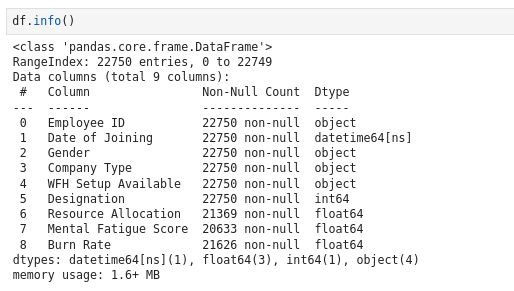
\includegraphics[width=0.8\textwidth]{Imagens/Grupo/info_grupo.png}
    \caption{Método \textit{info()}}
    \label{fig: info_grupo}
\end{figure}

Através do seguinte histograma podemos verificar que a nossa \textit{target} apresenta uma distribuição normal, o que beneficia as tomadas de decisão dos nossos modelos.

\begin{figure}[H]
    \centering
    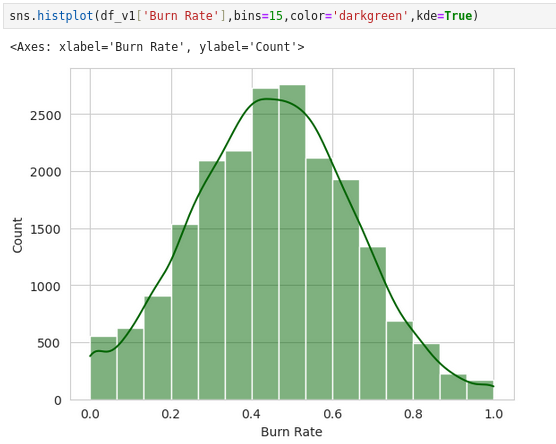
\includegraphics[width=0.7\textwidth]{Imagens/Grupo/histogram_grupo.png}
    \caption{Histograma referente à distribuição dos dados}
    \label{fig: histogram_grupo}
\end{figure}

Para ter uma melhor noção dos dados com que estávamos a trabalhar criamos mais alguns gráficos sendo o mais curioso o seguinte histograma:

\begin{figure}[H]
    \centering
    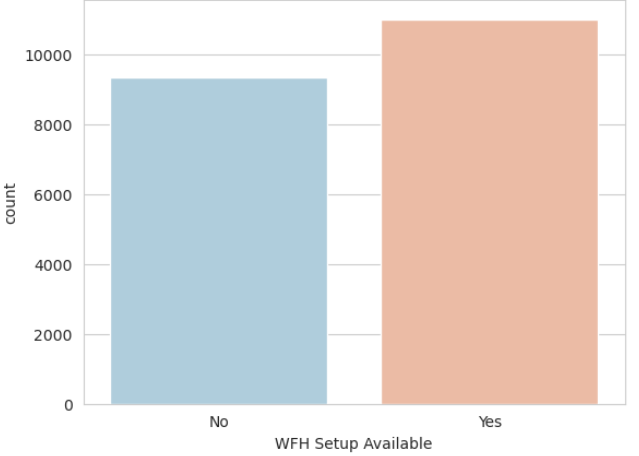
\includegraphics[width=0.7\textwidth]{Imagens/Grupo/local_trabalho.png}
    \caption{Local de trabalho}
    \label{fig: local_trabalho}
\end{figure}

Através deste podemos concluir que a maioria dos trabalhadores trabalha a partir de casa, algo que têm vindo a ser mais recorrente desde a época da pandemia COVID-19.

\begin{figure}[H]
    \centering
    \centerline{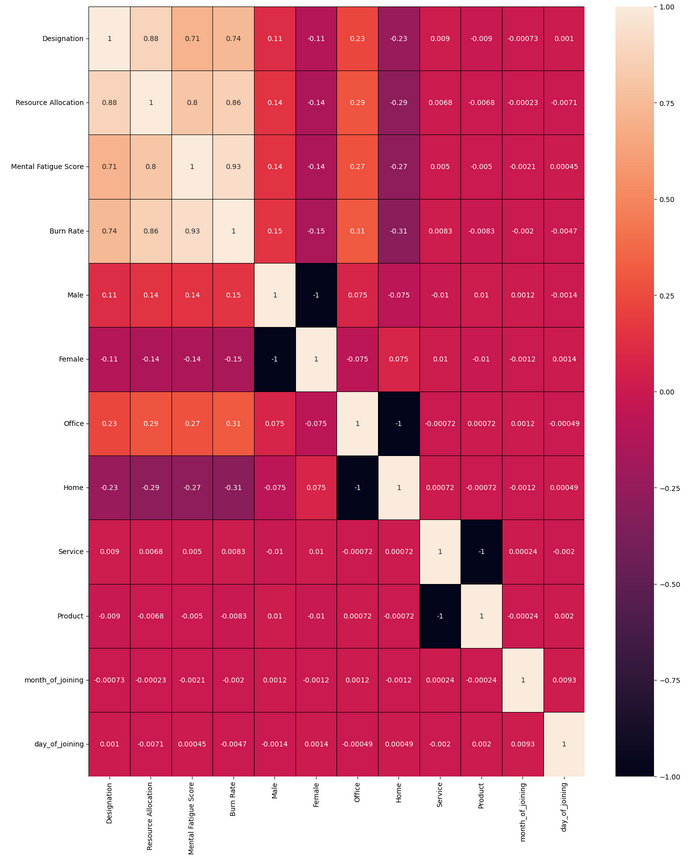
\includegraphics[width=1\textwidth]{Imagens/Grupo/matriz_correlacao_grupo.png}}
    \caption{Matriz de correlação}
    \label{fig: matriz_correlacao_grupo}
\end{figure}

Através do heatmap, podemos constatar algumas correlações entre os dados. Podemos constatar que a nossa \textit{label} tem forte correlação com outras 3 \textit{features} do \textit{dataset}, sendo eles Resource Allocation, Designation e a mais correlacionada, Mental Fatigue Score.

\begin{figure}[H]
    \centering
    \centerline{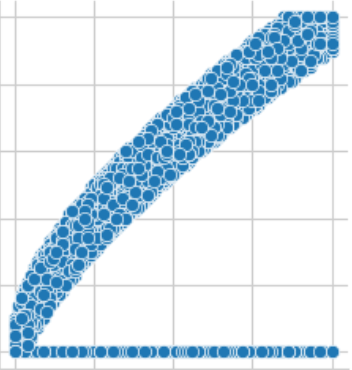
\includegraphics[width=0.5\textwidth]{Imagens/Grupo/seta.png}}
    \caption{Curva de regressão dos dados}
    \label{fig: grafico_azul_grupo}
\end{figure}

Esta última relação é também bem visível no histograma entre ambas no qual podemos tirar ainda a conclusão que embora muito perto, a Mental Fatigue score apresentada nem sempre coincide com o nível de burnout, portanto na sua previsão teremos de utilizar mais \textit{features}.

Foi ainda verificado nesta fase a existência de \textit{missing values} e a não existência de linhas duplicadas.

\begin{figure}[H]
    \centering
    \centerline{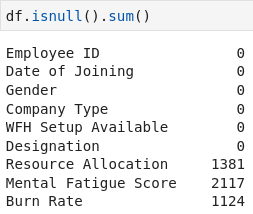
\includegraphics[width=0.5\textwidth]{Imagens/Grupo/missing_values_grupo.png}}
    \caption{\textit{Missing values}}
    \label{fig: missing_values_grupo}
\end{figure}

\section{Preparação de dados}
\paragraph{}
Uma vez que se verificou a existência de \textit{missing values} na fase de exploração, decidimos que as linhas com \textit{missing values} na coluna Burn Rate deviam ser retiradas, uma vez que esta é a nossa \textit{label}. O mesmo tratamento foi efetuado à Resource Allocation.
Para a Mental Fatigue Score não removemos, uma vez que a remoção de todas estas linhas iria equivaler a uma perda de cerca de 15\% dos dados. Por esta razão começamos por preencher os \textit{missing values} com 0, mas rapidamente abandonamos esta opção devido à visualização do gráfico da 'Curva de regressão de dados' anteriormente apresentado. Para um melhor "disfarce" da curva criamos uma função que preenche os \textit{missing values} tendo em conta uma terceira \textit{feature}, sendo decidida a Designation, por ter boa correlação, ficando a curva da seguinte maneira:

\begin{figure}[H]
    \centering
    \centerline{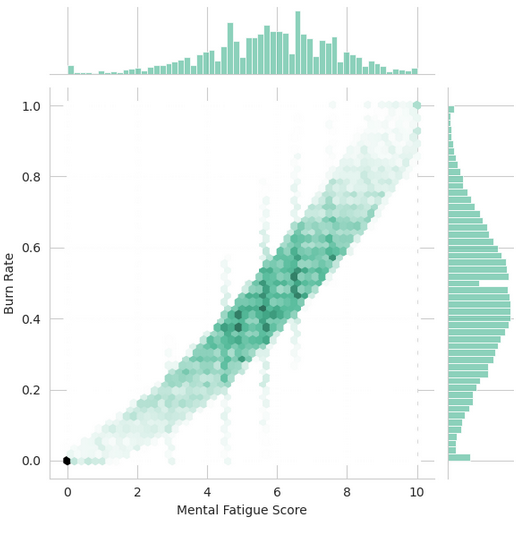
\includegraphics[width=0.7\textwidth]{Imagens/Grupo/curva_grupo.png}}
    \caption{Curva de regressão dos dados}
    \label{fig: curva_grupo}
\end{figure}

Decidimos de seguida retirar a coluna Employee ID, uma vez que é um valor distinto para cada linha e sendo que funciona como um identificador do trabalhador, não trás nenhuma informação relevante para o treino dos nossos modelos.

Para tratar dos dados categóricos foi utilizado one-hot encoding uma vez que os valores destas colunas têm pesos equivalentes e deste modo evitamos uma má influência durante o treino. As colunas que sofreram esta transformação foram: Gender, WFH Setup Available, e Company Type

\begin{minted}[fontsize=\footnotesize, xleftmargin=16pt, breaklines=true, breakanywhere=true]{python}
gender_mapper = {'Male': 0, 'Female': 1}
df_v1['Gender'] = df_v1['Gender'].replace(gender_mapper)
df_v1 = df_v1.join(pd.get_dummies(df_v1['Gender'], prefix='Gender').astype(int))
df_v1.rename(columns={'Gender_0': 'Male', 'Gender_1': 'Female'}, inplace=True)
df_v1.drop(['Gender'], axis=1, inplace=True)
\end{minted}

\begin{minted}[fontsize=\footnotesize, xleftmargin=16pt, breaklines=true, breakanywhere=true]{python}
workplace_mapper = {'No': 0, 'Yes': 1}
df_v1['WFH Setup Available'] = df_v1['WFH Setup Available'].replace(workplace_mapper)
df_v1 = df_v1.join(pd.get_dummies(df_v1['WFH Setup Available'], prefix='WFH Setup Available').astype(int))
df_v1.rename(columns={'WFH Setup Available_0': 'Office', 'WFH Setup Available_1': 'Home'}, inplace=True)
df_v1.drop(['WFH Setup Available'], axis=1, inplace=True)
\end{minted}

\begin{minted}[fontsize=\footnotesize, xleftmargin=16pt, breaklines=true, breakanywhere=true]{python}
company_mapper = {'Service': 0, 'Product': 1}
df_v1['Company Type'] = df_v1['Company Type'].replace(company_mapper)
df_v1 = df_v1.join(pd.get_dummies(df_v1['Company Type'], prefix='Company Type').astype(int))
df_v1.rename(columns={'Company Type_0': 'Service', 'Company Type_1': 'Product'}, inplace=True)
df_v1.drop(['Company Type'], axis=1, inplace=True)
\end{minted}

Foi ainda realizado \textit{feature engineering} na data para verificar se seria obtido mais informação.

Esta fase terminou com a remoção de todas as colunas relativas à data, uma vez que apresentavam uma correlação muito próxima de 0 com todas as outras \textit{features}. Foram ainda retiradas as colunas Product e Service, obtidas do one-hot encoding do Company Type, pelas mesmas razões apresentadas anteriormente.

\section{Modelação}

\subsection{Regressão Linear}
\paragraph{}
Para primeiro modelo, decidimos optar por um modelo simples e recorrentemente utilizado para problemas de regressão, a regressão linear. Tendo como objetivo prever o nível de burnout dos trabalhadores.
\begin{minted}[fontsize=\footnotesize, xleftmargin=16pt, breaklines=true, breakanywhere=true]{python}
lm = LinearRegression()
lm.fit(X_train, y_train)
\end{minted}

Assim sendo, obtivemos os seguintes resultados:
\begin{minted}[fontsize=\footnotesize, xleftmargin=16pt, breaklines=true, breakanywhere=true]{python}
MAE: 0.04872399285439895
MSE: 0.0038600687723920513
RMSE: 0.062129451730979016
\end{minted}

\subsection{Support Vector Regression}
\paragraph{}
Uma vez que utilizamos Support Vector para problemas de classificação nas aulas práticas, tentamos explorar a implementação destes modelos em problemas de regressão utilizando Support Vector Regression.

\begin{minted}[fontsize=\footnotesize, xleftmargin=16pt, breaklines=true, breakanywhere=true]{python}
svr = GridSearchCV(SVR(kernel='rbf'), param_grid={'C': [400,500,600], 'gamma': [1,0.01,0.0001]}, refit=True, verbose=3, scoring='neg_mean_absolute_error')
\end{minted}

Deste modo, obtivemos os seguintes resultados:
\begin{minted}[fontsize=\footnotesize, xleftmargin=16pt, breaklines=true, breakanywhere=true]{python}
MAE: 0.04954229400349311
MSE: 0.0039086508165031226
RMSE: 0.06251920358180454
\end{minted}

\subsection{Rede Neural Artificial}
\paragraph{}
Na implementação das redes neuronais artificiais partimos do modelo utilizado nas aulas práticas, realizando os ajustes necessários como, por exemplo, a dimensão de input.

A arquitetura final obtida pode ser observado de seguida. O modelo utilizado tem 4 camadas. A primeira possui então 7 neurónios relativos ao número de \textit{features}, as seguintes têm respetivamente 16,9 e 1.

\begin{minted}[fontsize=\footnotesize, xleftmargin=16pt, breaklines=true, breakanywhere=true]{python}
def build_model(activation='relu', learning_rate=0.01):
    model = Sequential()
    model.add(Dense(16, input_dim=7, activation=activation))
    model.add(Dense(9, activation=activation))
    model.add(Dense(1, activation=activation))
    
    model.compile(loss='mae', optimizer=tf.optimizers.Adam(learning_rate), metrics=['mae','mse'])
    return model
\end{minted}

\begin{minted}[fontsize=\footnotesize, xleftmargin=16pt, breaklines=true, breakanywhere=true]{python}
optimizer = ['SGD','RMSprop','Adagrad']
activation = ['sigmoid','relu']
param_grid = dict(optimizer=optimizer)
\end{minted}

\begin{minted}[fontsize=\footnotesize, xleftmargin=16pt, breaklines=true, breakanywhere=true]{python}
kf = KFold(n_splits=5, shuffle=True, random_state=2021)
\end{minted}

\begin{minted}[fontsize=\footnotesize, xleftmargin=16pt, breaklines=true, breakanywhere=true]{python}
model = KerasRegressor(model=build_model, batch_size=100, validation_split=0.2, epochs=80)
\end{minted}

\begin{minted}[fontsize=\footnotesize, xleftmargin=16pt, breaklines=true, breakanywhere=true]{python}
grid_search = GridSearchCV(estimator=model, param_grid=param_grid, cv=kf, scoring='neg_mean_absolute_error', refit='True', verbose=1)
\end{minted}

Para verificar se a arquitetura das redes neuronais não estavam a entrar em situação de overfitting, seguimos o exemplo da aula e criamos o seguinte gráfico:

\begin{figure}[H]
    \centering
    \centerline{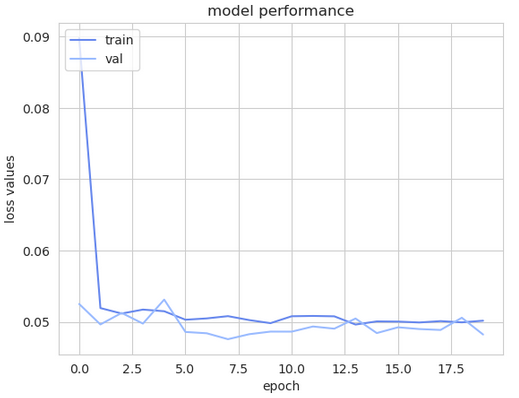
\includegraphics[width=0.7\textwidth]{Imagens/Grupo/ANN.png}}
    \label{fig: ANN}
\end{figure}

Após a sua análise consideramos que estamos na presença de um bom modelo.

Assim sendo, obtivemos os seguintes resultados:
\begin{minted}[fontsize=\footnotesize, xleftmargin=16pt, breaklines=true, breakanywhere=true]{python}
MAE: 0.048217227288524116
MSE: 0.0037480777355242247
RMSE: 0.06122154633398461
\end{minted}

\subsection{Gradient Boosting}
\paragraph{}
Criados os 3 últimos modelos decidimos partir para a implementação de um modelo sugerido pela professora durante o \textit{checkpoint}, o Gradient Boosting.

\begin{minted}[fontsize=\footnotesize, xleftmargin=16pt, breaklines=true, breakanywhere=true]{python}
param_boost = {'learning_rate': [0.01,0.02,0.03], 'subsample': [0.1, 0.2, 0.4], 'n_estimators': [128,256,512], 'max_depth': [4,8,12]}
\end{minted}

\begin{minted}[fontsize=\footnotesize, xleftmargin=16pt, breaklines=true, breakanywhere=true]{python}
estimator_boost = GradientBoostingRegressor()
grid_boost = GridSearchCV(estimator_boost, param_boost, refit=True, verbose=0)
\end{minted}

\begin{minted}[fontsize=\footnotesize, xleftmargin=16pt, breaklines=true, breakanywhere=true]{python}
{'learning_rate': 0.03, 'max_depth': 4, 'n_estimators': 512, 'subsample': 0.4}
\end{minted}

Finalmente, obtivemos os seguintes resultados para este último modelo:
\begin{minted}[fontsize=\footnotesize, xleftmargin=16pt, breaklines=true, breakanywhere=true]{python}
MAE: 0.045546670468378576
MSE: 0.00329982576622636
RMSE: 0.057444109935017355
\end{minted}

\section{Avaliação}
\paragraph{}
Após implementados os três modelos, realizamos então uma comparação entre os resultados obtidos.
Para obter uma perceção mais visual entre os MAE obtidos em cada um, criamos o seguinte gráfico de barras:

\begin{figure}[H]
    \centering
    \centerline{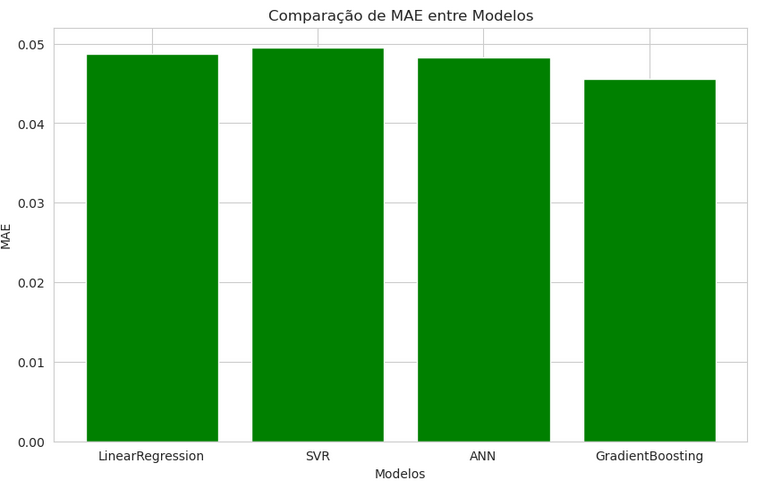
\includegraphics[width=1\textwidth]{Imagens/Grupo/MAE.png}}
    \label{fig: MAE}
\end{figure}

Como é possível observar, o modelo que apresentou melhor resultados foi o Gradient Boosting, no entanto, a diferença entre este resultado não é muito significativa quando comparado com os outros modelos.

Por outro lado, outro fator que podemos ter em conta é o tempo que cada um destes demorou para treinar e executar as previsões. Neste aspeto, a regressão linear ganha uma certa vantagem por ser mais simples e demorar cerca de 2 segundos para executar enquanto que os outros três modelos demoram 3 minutos ou mais.

Tendo estes dois fatores em conta, consideramos então que na necessidade de efetuar uma previsão o mais acertada possível, sem limites a nível de tempo, o modelo a ser utilizado deve ser o Gradient Boosting sendo o que apresentou melhores resultados.

Se as previsões tiverem de ser efetuadas o mais rápido possível e/ou os recursos disponíveis não forem os melhores possíveis, para estes casos, o grupo considera que a utilização de Regressão Linear é uma alternativa válida pois é um algoritmo mais leve e que obteve bons resultados, como podemos observar.

\chapter{Conclusão}
\paragraph{}
Após a conclusão deste trabalho prático, o grupo considera que os objetivos estabelecidos foram alcançados com sucesso. Os modelos desenvolvidos para os dois \textit{datasets}, um de classificação e outro de regressão, demonstraram um desempenho satisfatório, tanto no que diz respeito à precisão dos resultados como à relevância para os objetivos do projeto.

No que diz respeito ao \textit{dataset} da competição, o modelo de classificação desenvolvido foi capaz de prever com precisão a capacidade de produção de energia na rede elétrica em Braga, em kWh, para cada dia do ano. Este resultado permitiu ao grupo alcançar uma posição respeitável no ranking da competição Kaggle.

No caso do \textit{dataset} do grupo, desenvolvemos modelos de regressão com base nos dados cuidadosamente tratados e analisados, resultando num modelo capaz de prever o nível de burnout entre os trabalhadores. Estamos satisfeitos com a métrica de erro obtida, que consideramos bastante aceitável.

O grupo reconhece que há espaço para melhorias futuras, especialmente no que diz respeito ao refinamento e aprofundamento dos modelos apresentados neste relatório. No entanto, considera que os resultados alcançados são um bom ponto de partida para futuros projetos de Machine Learning.

Além disso, o grupo considera que o trabalho prático proporcionou uma oportunidade valiosa para aprofundar o conhecimento em relação às várias etapas de exploração, tratamento de dados e criação de modelos de aprendizagem automática. O grupo também desenvolveu competências no uso de Python Notebooks e em ambientes de desenvolvimento pelo Anaconda, que permitiram a realização deste projeto.


\end{document}
